\documentclass{article}

\setlength{\paperwidth}{210mm}
\setlength{\paperheight}{297mm}
\setlength{\hoffset}{-12mm}
\setlength{\voffset}{-10mm}
\setlength{\evensidemargin}{0mm}
\setlength{\oddsidemargin}{0mm}
\setlength{\topmargin}{0mm}
\setlength{\headheight}{0mm}
\setlength{\headsep}{5mm}
\setlength{\textheight}{256.2mm}
\setlength{\textwidth}{184.2mm}
\setlength{\marginparsep}{0mm}
\setlength{\marginparwidth}{0mm}
\setlength{\footskip}{5mm}
\setlength{\marginparpush}{0mm}


\usepackage[spanish]{babel}
\usepackage[utf8]{inputenc}
\usepackage{graphicx}

\pagestyle{myheadings}
\markright{IA - Práctica de búsqueda local}

\title{\Huge{Práctica de búsqueda local} \\
\vspace{15mm}
   \Large{Laboratorio de Inteligencia Artificial}}
\author{Marion Not - Michael Boris Mandirola}
\date{Primavera 2010-2011}

\begin{document}
\maketitle
\newpage
\tableofcontents
\newpage
\section*{Introducción}
El objetivo de esta práctica es analizar y resolver un problema de optimización
logística mediante algoritmos de búsqueda local. Definiremos la representación
del problema como estado y estudiaremos la influencia de los elementos que
intervienen en esta búsqueda y que hemos visto a clase (estado inicial, función
heurística y operadores) bajo diferentes condiciones sobre los parámetros del
problema.

Usaremos dos tipos de algoritmos de búsqueda local : el Hill Climbing y el
Simulated Annealing. Como el objetivo de la práctica no es la implementación de
estos algoritmos, usaremos las herramientas proporcionadas por el package AIMA. 
En el caso del Simulated Annealing, también estudiaremos la influencia de los 
parámetros del algoritmo.

\section{Representación del problema}
El contexto del problema es el siguiente : Una empresa de transporte está
contratada por una compañía para gestionar el encaminamiento de productos desde
un almacén central hasta unos centros de producción.

Cada día, los centros realizan un conjunto de peticiones de diferentes tipos y 
cantidades de productos que se tienen que entregar a una cierta hora. El pago se
realiza en función de la cantidad de productos entregados y la puntualidad con
la cual han llegado al centro.

La empresa de transporte quiere optimizar estas entregas, sabiendo que manda un
transporte a cada centro en cada hora en punto del día.
No tenemos que gestionar la recogida de productos en el almacén, ni el recorrido
de los transportes, ni la cantidad de camiones físicos que se necesitan :
Suponemos que la empresa dispone de una flota suficiente para hacer todas las
entregas en tiempo.
Solucionaremos este problema para un solo día, pues las peticiones no entregadas
no estarán desplazadas al día siguiente.

\subsection{Identificación de los elementos relevantes}
Para cada problema, tendremos unos elementos constantes, unos elementos
específicos del problema y unos elementos variables que se tendrán que
determinar para llegar a la solución.

\subsubsection{Constantes}
\begin{description}
\item[Centros de producción :] Como lo hemos dicho, el número de centros esta 
fijado a 6.
\item[Horas de entrega :] Las entregas se harán a cada hora en punto del día. La
primera se hará a las 8 y la última a las 17, para un total de 10 horas de
entrega.
\item[Transportes :] Tendremos un transporte para cada hora del día y cada
centro, es decir 60 transportes en total. La capacidad de los camiones usados
sera de 500, 1000 o 2000kgs, en proporción variable.
\item[Peticiones :] Las peticiones se harán para una de las horas de entregas y
para una cantidad de productos de 100, 200, 300, 400 o 500kgs.
\end{description}

\subsubsection{Elementos específicos del problema}
\begin{description}
\item[Peticiones :] Todas las peticiones estarán generadas al principio de la
resolución mediante unos parámetros especificados por el usuario. Por lo tanto,
serán diferentes para cada problema. Se tendrán que especificar :
\begin{itemize}
\item El número de peticiones
\item La distribución de probabilidad de cantidad de productos de las entregas
\item La distribución de probabilidad de horas de entrega
\end{itemize}
Las peticiones estarán repartidas de forma equiprobable entre los centros.
El tipo de producto pedido no tienen ninguna influencia.
\item[Transportes :] Se tendrá que especificar la distribución de probabilidad
de capacidades de los transportes, es decir cuantos de los 60 transportes
tendrán una capacidad de 500kgs, cuantos de 1000 y cuantos de 2000.
\item[Parámetros de la búsqueda :] Se precisará que tipo de estado inicial,
algoritmo de búsqueda y función heurística se tienen que usar. 
\end{description}

\subsubsection{Elementos de la solución}
Para llegar a la solución, se tendrán que determinar :
\begin{itemize}
\item La repartición de los 60 transportes, es decir que capacidad de transporte
se asignará à cada hora de cada centro.
\item La repartición de las peticiones en los transportes.
\end{itemize}

\subsection{Definición del Estado}
Hemos escogido una representación en acuerdo con la decripción del problema de
la parte anterior.
\subsubsection{Implementación}
\begin{center} 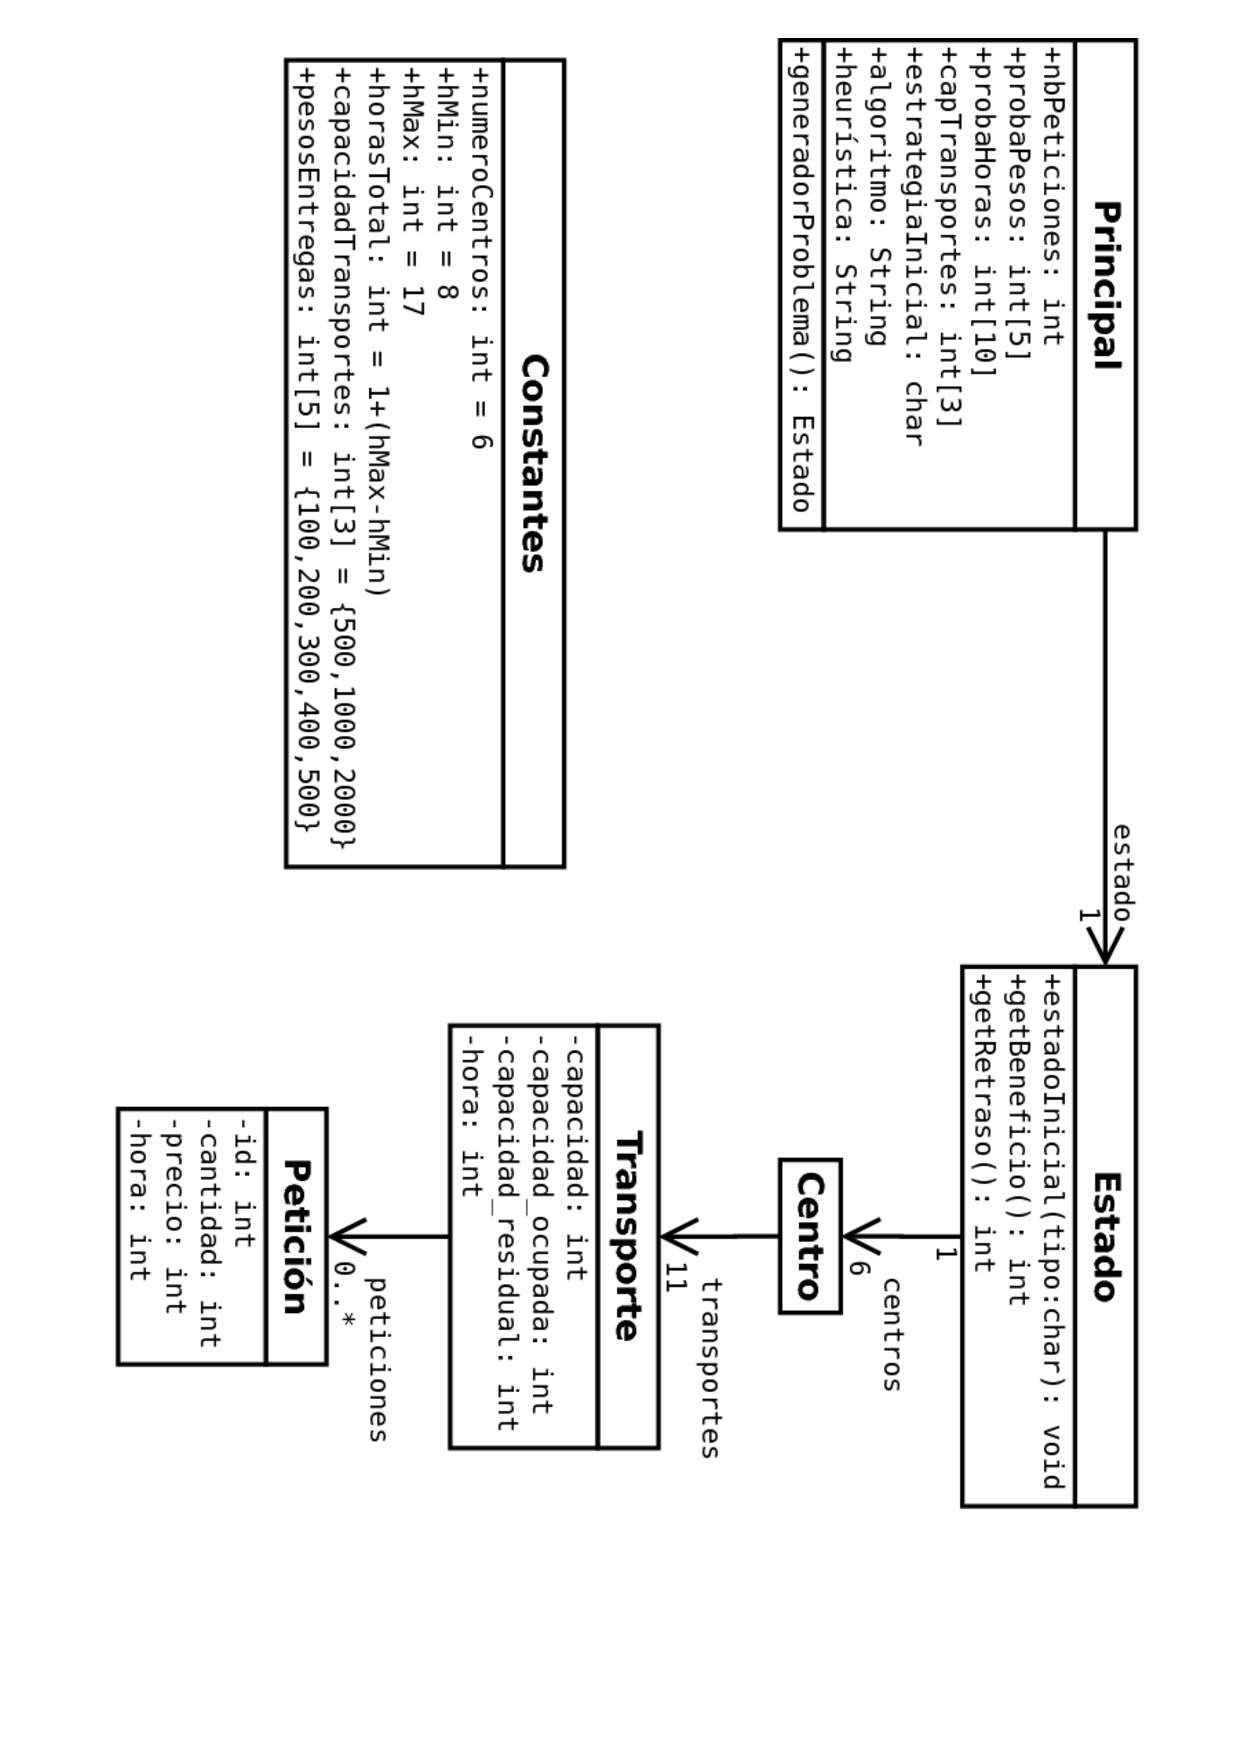
\includegraphics[width=14cm, angle=90]{clases}\\
{\it Fig. 1 : Diagrama de clases de representación del problema} \end{center}
\begin{itemize}
\item Una clase singleton Constantes contiene los elementos comunes a todos los
problemas.
\item Los elementos especificos serán leidos desde un fichero .txt y usados por
el Principal para generar un problema dado, es decir un conjunto de instancias
de la clase Petición y un Estado ``vacio'', donde las peticiones estarán
repartidas entre las 6 instancias de clase Centro pero no entregadas. Se crearán
11 instancias de clase Transporte : una para cada hora del día y una para
guardar las peticiones no entregadas.
\item A continuación, se generará el estado inicial de la búsqueda, es decir que
se atribuirá una capacidad a cada unos de los 60 transportes que corresponden a
una hora (los Transporte de peticiones no entregadas tendrán capacidad máxima) y
se repartirán las peticiones según la estrategia especificada.
\item Durante la resolución del problema, las peticiones se desplazarán de un
Transporte a otro, dentro del mismo Centro. Tambien se podrá modificar la
repartición de las capacidades entre todos los 60 transportes. Ver la sección
siguiente para detalles sobre los operadores.
\end{itemize}
\subsubsection{Tamaño del espacio de búsqueda}
Si tenemos $N$ peticiones, repartidas igualmente entre 6 centros ($\frac{N}{6}$
peticiones/centro), que se pueden afectar a cualquier de los $10+1$ transportes,
contamos con $O(11^N)$ configuraciones posibles para la repartición de las
peticiones.\\
Si añadimos que cada uno de los 60 transportes puede tener una de 3 capacidades,
es decir $O(3^{60})$ configuraciones posibles, tenemos un total de
\textbf{$O(11^Nx3^{60})$ estados posibles}.\\
\indent Se tiene que tener en cuenta que en verdad la suma de pesos de las
peticiones afectadas a un transporte no puede exceder su capacidad, y que
tenemos un número limitado de transportes de cada capacidad : Eso reduce el
tamaño del espacio de búsqueda.\\
\indent Este tamaño es bastante importante, pero considerando que hacemos una
búsqueda local y que recorriremos solo una fracción del espacio, no es excesivo.

\subsection{Operadores}
%descripcion detallada, condiciones de aplicacion, efecto
%factor de ramificacion
%justificacion de la eleccion
\subsubsection{Desplazamiento de una petición dentro de un centro}
\subsubsection{Intercambio de capacidades de camiones}
\subsubsection{Operadores no implementados}


\subsection{Funciones Heurísticas}
%descripcion y analisis de los factores que intervienen en las heuristicas
%justificacion de la eleccion de estas heuristicas y de las ponderaciones
%explicacion del impacto de las heuristicas en la busqueda
\subsubsection{Maximización de la ganancia}
\begin{description}
\item[Definición de la ganancia :]
Para cada petición, la compañia pagará a la empresa de transporte un importe
basado sobre el precio base de las peticiones (indicado en la tabla 1), que
depende unicamente de la cantidad de productos pedida, y la puntualidad de la 
entrega.\\
\begin{center}
\begin{tabular}{|l|l|}
\hline
Peso & Precio\\
\hline
100 y 200 kg & {\it peso} euros\\
300 y 400 kg & 1,5x{\it peso} euros\\
500 kg & 2x{\it peso} euros\\
\hline
\end{tabular}\\
{\it Tabla 1 : Precio base de las entregas.} \end{center}
El importe pagado para cada petición entregada será el precio base menos unos
20\% del mismo para cada hora de retraso, es decir que para mas de 5h de retraso
le tocara pagar a la empresa de transporte. Si una petición no esta entregada enel día, la empresa de transporte tendrá que pagar el precio base de la petición
mas unos 20\% del mismo para cada hora hasta las 17.\\

Ejemplo : Para cada peso de petición, en la tabla 2 se indican los
importes correspondientes a una entrega en tiempo, una entrega con 1 y 7 horas
de retraso y no entrega, considerando que las peticiones se tenián que entregar
a las 10.
\begin{center}
\begin{tabular}{|l|l|l|l|l|l|l|}
\hline
Peso & En tiempo ($<$10h) & Retraso 1h (=11h) & Retraso 7h (=17h) &
No entregada\\
\hline
100kg & 100 & 80 & -40 & -240\\
200kg & 200 & 160 & -80 & -560\\
300kg & 450 & 360 & -180 & -1080\\
400kg & 600 & 480 & -240 & -1440\\
500kg & 1000 & 800 & -400 & -2800\\
\hline
\end{tabular}\\
{\it Tabla 2 : Ejemplos de importes.} \end{center}
\end{description}

\subsubsection{Minimización de la diferencia entre hora de entrega deseada y
efectiva}
El retraso en la entrega de una petición es simplemente la diferencia entre la
hora de entrega deseada y la efectiva. Si la petición no esta entregada en el
día, el retraso es la diferencia entre la hora de entrega deseada y las 8 del
día siguiente. No obstante, como solucionemos el problema solo para una jornada,
no se tendra que gestionar la entrega de estas peticiones.

\subsection{Estados Iniciales}
%justificacion de la eleccion de los estados (bondad de la solucion, coste,
% adaptacion a cada algoritmo)
%descripcion de la implementacion

En un primer momento hemos intentado generar estados diferentes con lógicas muy diferentes con la idea de buscar nuestros estados iniciales entre un grupo más amplio y en particular elegir dos estados que tengan características muy diferentes. Es decir tiempo de generación de el estado inicial, complejidad de el algoritmo, posibilidades de evolución, calidad de la solución buscada.

\subsubsection{a}
A) Este estado divide los camiones de manera ecua entre los centres asignando los camiones con mas capacidad a los transportes mas tempranos. Las entregas están entregadas lo mas pronto posible: se hace una lista de peticiones pertinentes a un centro, se ordenan crecientemente por tiempo de entrega y disminuyendo por precio y se pasa toda la lista poniendo las peticiones en el transporte más pronto que tiene más tiempo libre.

\subsubsection{b}
B) Este estado ordena las peticiones por precio y hora. Por cada petición, intenta entregarla en la hora pertinente con este algoritmo:
Si no hay camión, se pone el camión disponible más pequeño y la petición, si hay camión y bastante capacidad libre también se pone la petición. Si hay camión de capacidad inferior a la capacidad máxima y hay disponibilidad de camiones más grandes, se asigna un camión mas grande en lugar de lo más pequeño y se pone la petición. Además, si no hay camiones libres más grandes intenta hacer lo mismo en las horas más tempranas hasta las 8. Si no tiene éxito, intenta hacerlo en las horas después hasta las 17.
Después si hay oras sin camión, se asignan los camiones que se quedan libres.

\subsubsection{f}
F) Los camiones se asignan como en el estado A. Sin ordinación se iteran todas las peticiones intentando ponerlas en su hora de pertinencia. Después, iterativamente por cada petición se intenta poner, las que se quedan no entregadas, en las horas más tempranas de la suya hasta las 8 y si no se tiene éxito, se intenta hacerlo en las horas después hasta las 17.

\subsubsection{v}
V) Los camiones se asignan como en el estado A. Las peticiones se quedan todas no entregadas.


\section{Implementación}

\subsection{Generación de problemas aleatorios}

\subsection{Uso del AIMA}

\subsection{Ejecución de pruebas}
El programa efectúa las pruebas sacando los parametros necesarios de ficheros de texto. Los ficheros estan organizados en la siguiente manera:
\begin{itemize}
\item Linia 1 : Numero de pruebas con estos parametros - 1 Integer
\item Linia 2 : Numero de peticiones - 1 Integer
\item Linia 3 : Distribucion de capacidad de los camiones - 3 Integers para 500, 1000 y 2000kg - La suma de los 3 debe ser igual a 60.
\item Linia 4 : Distribucion de pesos de las peticiones - 5 Floats para 100 hasta 500kg - La suma de los 5 debe ser igual a 1.
\item Linia 5 : Distribucion de las horas de entrega - 10 Floats para 8h hasta 17h - La suma de los 10 debe ser igual a 1.
\item Linia 6 : Estrategia para generar el estado inicial - 1 Char
\item Linia 7 : Tipo de algoritmo - String - Puede ser "hc" o "sa".
\item Linia 8 : Tipo de heuristica - String - Puede ser "gan" o "ret".
La separacion entre la parte entera y decimal puede ser una coma (,) o un punto (.), si sale un error "formato no valido", intenta cambiar eso.
\end{itemize}
Cada experimento, pero, necesita una batería de pruebas con diferentes parametros. Así tenemos una carpeta para cada experimento con diferentes ficheros para generar pruebas. Un {\it bash script} recibe en input el numero de el experimento y resuelbe el problema con los ficheros de prueba pertinentes.

\subsection{Recuperación de resultados}
%output
Por cada problema son generados dos ficheros de salida, uno con el estado inicial y el otro con el estado final. En estos ficheros tenemos:
\begin{itemize}
\item El beneficio
\item El retraso
\item Los centros y por cada centro
	\begin{itemize}
		\item Cantidad de peticiones no entregadas
		\item Las horas y por cada hora de entrega
		\begin{itemize}		
			\item La capacidad total
			\item La capacidad ocupada
			\item La capacidad libre
			\item Las peticiones no entregadas y por cada petición		
			\begin{itemize}
			\item El identificador
			\item La hora de entrega supuesta
			\item La cantidad
			\item El precio
			\end{itemize}
		\end{itemize}
	\end{itemize}
\end{itemize}
También hay un fichero de estadísticas por cada experimento a que vamos anadiendo datos sobre las pruebas. Este fichero está organizado como un CSV y por cada prueba tenemos registrados:
\begin{itemize}
\item El numero de nodos desarrollados. 
\item El beneficio.
\item El percentaje de mejoría de el beneficio.
\item El retraso
\item El percentaje de mejoría de el retraso.
\item El tiempo de ejecución de la búsqueda.
\end{itemize}
Una linea vacía y una linea con el título del fichero de input dividen los diferentes grupos de pruebas (resultado de diferentes ejecuciones de el programa).

\section{Resultados}
% explicaciones y analisis detallada
% comparar los resultados con lo que se esperaba
% hacer los experimentos del enunciado y contestar las preguntas
% hacer tb mas experimentos para complementar

\subsection{Influencia de la solución inicial}
%coste de creacion
% influenca en la bondad de la solucion y en el coste del algoritmo

\subsection{Influencia de los operadores}
% comparacion entre conjuntos de operadores
% impacto sobre el coste temporal y bondad de la solucion

\subsection{Influencia de la heurística}
% comparacion entre las dos heuristicas, impacto en tiempo y bondad de solucion
% hacer experimentos para ver la influenca de las ponderaciones

\end{document}
